\chapter{Pumping Lemma}

Il pumping lemma stabilisce una condizione necessaria affinché
un linguaggio sia regolare.

Questo significa che ogni linguaggio regolare deve verificare la
proprietà espressa dal pumping lemma.
Ma se un linguaggio verifica il pumping lemma non è detto
che sia regolare.

\subsubsection{Pumping Lemma}

Sia $L$ un linguaggio regolare sull'alfabeto $\Sigma$. 

Esiste un numero $p$ (detto la lunghezza del pumping o la costante del pumping) tale che se $w$ è una qualsiasi stringa in $L$ di lunghezza almeno $p$, allora $w$ può essere divisa in tre sottostringhe, $w=x y z$ soddisfacenti le seguenti condizioni:
\begin{enumerate}
    \item $|x y| \leq p$
    \item $y \neq \epsilon$
    \item per ogni $k \geq 0, x y^{k} z \in L$
\end{enumerate}

Ogni linguaggio finito verifica il pumping lemma.

Nella prova si pone $p$ uguale al numero degli stati di un DFA che riconosce $L$.
Se $w \in L$ e $|w| \geq p$, allora $w=a_{1} \cdots a_{m}$ con $a_{i} \in \Sigma$ per $i=1, \ldots, m$ e $m \geq p$.
L'insieme $\left\{\hat{\delta}\left(q_{0}, a_{1} \cdots a_{i}\right) \mid 0 \leq i \leq m\right\}$ ha al più $p$ elementi ma ci sono $m+1$ "relazioni" $r_{i}=\hat{\delta}\left(q_{0}, a_{1} \cdots a_{i}\right)$, con $m+1>p$. Si considerano le prime $p+1$ relazioni $r_{0}, r_{1}, \ldots, r_{p}$.

\begin{figure}[hbpt!]
    \centering
    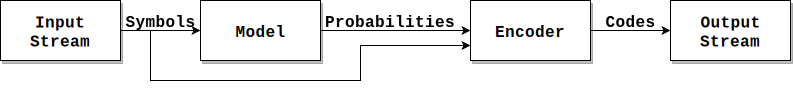
\includegraphics[width=6cm]{./Images/5.1.png}
\end{figure}
\FloatBarrier

La non regolarità di un linguaggio L a volte
viene stabilita mostrando che L non verifica il pumping lemma.

\vspace{5mm}

Per provare che $L$ non soddisfa il pumping lemma occorre provare che per ogni intero $p$ esiste una stringa $w \in L$ con $|w| \geq p$ tale che per ogni fattorizzazione $w=x y z$ con $y \neq \epsilon \mathrm{e}|x y| \leq p$, esiste $k \geq 0$ tale che $x y^{k} z \notin L$.
\begin{itemize}
    \item Non si può scegliere $p$.
    \item Si può scegliere $w$.
    \item Non si può scegliere la particolare fattorizzazione di $w$. Bisogna provare che nessuna fattorizzazione possibile di $w$ verifica le tre condizioni.
\end{itemize}

\subsubsection{Esercizio 1}

Mostriamo che
$$
\left\{b^{n} c^{n} \mid n \geq 0\right\}
$$
non soddisfa il pumping lemma.

\vspace{5mm}

Per assurdo, sia $p$ la costante del pumping lemma e consideriamo $b^{p}c^{p} \in L$. Ovviamente $\left|b^{p}c^{p}\right| \geq p$.


Esiste quindi una suddivisione $b^{p}c^{p}=x y z$ con $|x y| \leq p, y \neq \epsilon$ e $x y^{k} z \in L$ per ogni $k \in \mathbb{N}$.


Quindi $y=b^{r}$ con $0<r \leq p$.
Allora $x z=b^{p-r}c p \notin L$, essendo $p-r<p .$ Contraddizione.

\subsubsection{Esercizio 2}

Mostriamo che
$$
\left\{a b^{n} c^{n} \mid n \geq 0\right\}
$$
non soddisfa il pumping lemma.

\vspace{5mm}

Per assurdo, sia $p$ la costante del pumping lemma e consideriamo $a b^{p}c^{p} \in L$. Ovviamente $\left|a b^{p}c^{p}\right| \geq p$.
Esiste quindi una suddivisione $a b^{p}c^{p}=x y z \operatorname{con}|x y| \leq p$, $y \neq \epsilon \mathrm{e} x y^{k} z \in L$ per ogni $k \in \mathbb{N}$.

Sono possibili solo due casi:
\begin{enumerate}
    \item $x=\epsilon, y=a b^{r}$ con $0 \leq r<p$
    \item $x \neq \epsilon, y=b^{r}$ con $0<r<p$.
\end{enumerate}

Nel primo caso, $x z=b^{p-r}c^{p} \notin L$. Nel secondo caso $x z=a b^{p-r}c^{p} \notin L$ perché $p-r<p$. Contraddizione.

\subsubsection{Esercizio 3}

Sia $L=\left\{x c y \mid x, y \in\{a, b\}^{*}, x\right.$ e $y$ hanno lo stesso numero di a o $x$ e $y$ hanno lo stesso numero di $b\}$.
Ad esempio, acaa, abcab $\in$ L ma acb $\notin L$.
Provare o confutare che $L$ è regolare.

\vspace{5mm}

\textbf{Soluzione:}

L non è regolare. Infatti, supponiamo per assurdo che lo sia. Sia $n$ la costante del pumping lemma.

Consideriamo $a^{n} b c a^{n} b b$.

Poiché $a^{n} b c a^{n} b b \in L$ e $\left|a^{n} b c a^{n} b b\right| \geq n$, risulta $a^{n} b c a^{n} b b=x y z \operatorname{con}|x y| \leq n, y \neq \epsilon \mathrm{e} x y^{k} z \in L$ per ogni $k \in \mathbb{N}$.

Quindi, $x y=a^{p}$ e $y=a^{q}$ con $q \neq 0$.

Dovremmo avere $x y^{0} z=a^{n-q} b c a^{n} b b \in L$, con $n-q \neq n$, perché $q \neq 0$.
Questo è impossibile perché $a^{n-q} b$ e $a^{n} b b$ non hanno né lo stesso numero di a né lo stesso numero di $b$.

\subsubsection{Esercizio 4}

Siano $x, y \in \Sigma^{*}$. Diciamo che $y$ è fattore di $x$ se esistono $z, z^{\prime} \in \Sigma^{*}$ tali che $x=z y z^{\prime}$.

Dimostrare che il linguaggio
$$
L=\left\{x c y \mid x, y \in\{a, b\}^{*} \text { e y è fattore di } x\right\}
$$
non è regolare.

Giustificare la risposta.

\vspace{5mm}

\textbf{Soluzione:}

Supponiamo per assurdo che $L=\left\{x c y \mid x, y \in\{a, b\}^{*}\right.$ e $y$ è fattore $\left.\mathrm{di} x\right\}$ sia regolare. Sia $n$ la costante del pumping lemma. Consideriamo la stringa $a^{n} c a^{n}$.

Poiché $a^{n} c a^{n} \in L$ e $\left|a^{n} c a^{n}\right| \geq n$, risulta $a^{n} c a^{n}=x y z$ con $|x y| \leq n, y \neq \epsilon \mathrm{e} x y^{k} z \in L$ per ogni $k \in \mathbb{N}$.

Quindi, $x y=a^{p}$ e $y=a^{q}$ con $q \neq 0$.

Dovremmo avere $x y^{0} z=a^{n-q} c a^{n} \in L$, con $n-q<n .$ Questo è assurdo perché $a^{n}$ non può essere fattore di $a^{n-q}$, essendo $n-q<n .$

\subsubsection{Esercizio 5}
Mostrare che il linguaggio
$$
\cup_{k \geq 0}\left(a^{+} c\right)^{k}\left(b^{+} c\right)^{k}
$$
non è regolare.

\vspace{5mm}

\textbf{Soluzione:}

Supponiamo per assurdo che $L=\cup_{k \geq 0}\left(a^{+} c\right)^{k}\left(b^{+} c\right)^{k}$ sia regolare e sia $n$ la costante del pumping lemma.

Consideriamo la stringa $(a c)^{n}(b c)^{n}$.

Poiché $(a c)^{n}(b c)^{n} \in L$ e $\left|(a c)^{n}(b c)^{n}\right| \geq n$, risulta $(a c)^{n}(b c)^{n}=x y z$ con $|x y| \leq n, y \neq \epsilon \mathrm{e} x y^{k} z \in L$ per ogni $k \in \mathbb{N}$.
Quindi $x y$ è un prefisso di $(a c)^{n}$ e $x y^{0} z=x z=w^{\prime}(b c)^{n} \in L$.

Distinguiamo due casi: $|y|_{c}>0$ oppure $|y|_{c}=0$.
\begin{itemize}
    \item Se $|y|_{c}>0$ allora $\left|w^{\prime}\right|_{c}<n$ e quindi $w^{\prime} \notin\left(a^{+} c\right)^{n}$, assurdo.
    \item Se $|y|_{c}=0$ allora $y=a$. Quindi $\left|w^{\prime}\right|_{a}<n$ e di conseguenza $w^{\prime} \notin\left(a^{+} c\right)^{n}$, assurdo.
\end{itemize}

\subsubsection{Esempio}

Il linguaggio
$$
L=\left\{a^{i} b^{j} c^{k} \mid i, j, k \geq 0 \text { e se } i=1 \text { allora } j=k\right\}
$$
non è regolare.

Per provarlo si utilizza la proprietà di chiusura dei linguaggi regolari rispetto all'intersezione.

Osserviamo che
$$
L=\left\{a b^{n} c^{n} \mid n \geq 0\right\} \cup L\left(\left(\epsilon+a^{2} a^{*}\right) b^{*} c^{*}\right)
$$

\vspace{5mm}

II linguaggio $L\left(a b^{*} c^{*}\right)$ è regolare. Se $L$ fosse regolare lo sarebbe anche
$$
L \cap L\left(a b^{*} c^{*}\right)=\left\{a b^{n} c^{n} \mid n \geq 0\right\} .
$$
Ma abbiamo provato che
$$
\left\{a b^{n} c^{n} \mid n \geq 0\right\}
$$
non soddisfa il pumping lemma e quindi $L \cap L\left(a b^{*} c^{*}\right)$ non è regolare.

Di conseguenza nemmeno
$$
L=\left\{a b^{n} c^{n} \mid n \geq 0\right\} \cup L\left(\left(\epsilon+a^{2} a^{*}\right) b^{*} c^{*}\right)
$$
è regolare.

\vspace{5mm}

Il linguaggio
$$
\begin{aligned}
L &=\left\{a^{i} b^{j} c^{k} \mid i, j, k \geq 0 \text { e se } i=1 \text { allora } j=k\right\} \\
&=\left\{a b^{n} c^{n} \mid n \geq 0\right\} \cup L\left(\left(\epsilon+a^{2} a^{*}\right) b^{*} c^{*}\right)
\end{aligned}
$$
soddisfa le condizioni del Pumping Lemma per i linguaggi regolari, pur non essendo regolare. (Scegliendo come costante del pumping $p=2)$.

\vspace{5mm}

\textbf{Soluzione:}

$$
L=\left\{a b^{n} c^{n} \mid n \geq 0\right\} \cup L\left(\left(\epsilon+a^{2} a^{*}\right) b^{*} c^{*}\right)
$$
Dimostriamo che $L$ soddisfa il pumping lemma scegliendo come costante $n=2$.

Consideriamo i possibili casi possibili per una stringa in $L$ di lunghezza maggiore o uguale a 2 e facciamo vedere che per ognuno di tali casi esiste una suddivisione che verifica le condizioni del lemma.

Se $w \in L$ e $|w| \geq 2$, per $w$ sono possibili i seguenti casi
\begin{itemize}
    \item $w=a b^{n} c^{n}$, con $n>0$
    \item $w=a a b^{j} c^{t}$, con $j \geq 0, t \geq 0$
    \item $w=a^{r} b^{j} c^{t}$, con $r>2, j \geq 0, t \geq 0$
    \item $w=b^{j} c^{t}, \operatorname{con} j \geq 1 e j+t \geq 2$
    \item $w=c^{t}$, con $t \geq 2$
\end{itemize}

\vspace{5mm}

Se $w=a b^{n} c^{n}$, con $n>0$, prendiamo $x=\epsilon, y=a$. Le condizioni del lemma sono verificate:
$$
\begin{aligned}
&|x y|=1 \leq 2, \\
&|y|=1>0, \\
&x y^{k} z=a^{k} b^{n} c^{n} \in L, \text { per ogni } k \geq 0 .
\end{aligned}
$$

\vspace{5mm}

Se $w=a a b^{j} c^{t}$, con $j \geq 0, t \geq 0$, prendiamo $x=\epsilon, y=a a .$
Le condizioni del lemma sono verificate:
$|x y|=2 \leq 2$, $|y|=2>0$, $x y^{k} z=(a a)^{k} b^{j} c^{t} \in L$, per ogni $k \geq 0 .$

\vspace{5mm}

Se $w=a^{r} b^{j} c^{t}$, con $r>2$, con $j \geq 0, t \geq 0$, prendiamo $x=\epsilon$,
$y=a .$

Le condizioni del lemma sono verificate:
\begin{itemize}
    \item $|x y|=1 \leq 2$
    \item $|y|=1>0$
    \item $x y^{k} z=a^{r+k-1} b^{j} c^{t} \in L$, per ogni $k \geq 0$
\end{itemize}

Se $w=b^{j} c^{t}$, con $j \geq 1, j+t \geq 2$, prendiamo $x=\epsilon, y=b .$
Le condizioni del lemma sono verificate:
\begin{itemize}
    \item $|x y|=1 \leq 2$
    \item $|y|=1>0$
    \item $x y^{k} z=b^{j+k-1} c^{t} \in L$, per ogni $k \geq 0$
\end{itemize}

Se $w=c^{t}$, con $t \geq 2$, prendiamo $x=\epsilon, y=c$

Le condizioni del lemma sono verificate:
\begin{itemize}
    \item $|x y|=1 \leq 2$
    \item $|y|=1>0$
    \item $x y^{k} z=c^{t+k-1} \in L$, per ogni $k \geq 0$
\end{itemize}

\vspace{5mm}

Si consideri il linguaggio $L$ definito come segue:
$$
\begin{aligned}
L=&\{a, b, c\}^{*} c c\{a, b, c\}^{*} \cup \\
& \cup_{k \geq 0}\left(a^{+} c\right)^{k}\left(b^{+} c\right)^{k} \\
=&\{a, b, c\}^{*} c c\{a, b, c\}^{*} \cup \\
&\left\{w \in\{a, b, c\}^{*} \mid \exists k \geq 0, \exists n_{1}, \ldots n_{k}, m_{1}, \ldots, m_{k} \geq 0\right.\\
& \text { tali che } w=a^{\left.n_{1} c \cdots a^{n_{k}} c b^{m_{1}} c \cdots b^{m_{k}} c\right\}}
\end{aligned}
$$
Ad esempio, $a c c b, a c a^{2} c b^{3} c b c \in L$ e acbcbbc $\notin L$. L non è regolare ma soddisfa le condizioni del Pumping Lemma per i linguaggi regolari (scegliendo come costante del pumping $p=3$ ).

\vspace{5mm}

$$
\begin{aligned}
&L=\{a, b, c\}^{*} c c\{a, b, c\}^{*} \cup\left(\cup_{k \geq 0}\left(a^{+} c\right)^{k}\left(b^{+} c\right)^{k}\right) \\
&L_{1}=\{a, b, c\}^{*} c c\{a, b, c\}^{*} \text { è regolare. }
\end{aligned}
$$

Utilizzando il pumping lemma abbiamo provato che $L_{2}=\cup_{k \geq 0}\left(a^{+} c\right)^{k}\left(b^{+} c\right)^{k}$ non è regolare.
$L_{1} \cap L_{2}=\emptyset$

Se $L$ fosse regolare lo sarebbe anche $L-L_{1}=L_{2}$ e questo non è vero. Quindi $L$ non è regolare.

Dimostriamo che $L$ soddisfa il pumping lemma scegliendo come costante $n=3$.

Consideriamo i possibili casi possibili per una stringa in $L$ di lunghezza maggiore o uguale a 3 e facciamo vedere che per ognuno di tali casi esiste una suddivisione che verifica le condizioni del lemma.

Se $w \in L$ e $|w| \geq 3$, per $w$ sono possibili i seguenti casi
\begin{itemize}
    \item $w=z_{1} c c z_{2}$, con $z_{1} z_{2} \neq \epsilon$.
    \item $w \in\left(a^{+} c\right)^{k}\left(b^{+} c\right)^{k},|w| \geq 3$ e $w$ inizia con aca. Quindi $w=a c a^{j} c w^{\prime}, j \geq 1$.
    \item  $w \in\left(a^{+} c\right)^{k}\left(b^{+} c\right)^{k},|w| \geq 3$ e w inizia con acb. Quindi $w=a c b^{j} c, j \geq 1$.
    \item $w \in\left(a^{+} c\right)^{k}\left(b^{+} c\right)^{k},|w| \geq 3$ e $w$ inizia con $a^{j} c, j \geq 2$.
    \item $w=z_{1} c c z_{2}$, con $z_{1} z_{2} \neq \epsilon .$ Se $z_{1}=\sigma z^{\prime}, \sigma \in\{a, b, c\}$
prendiamo $x=\epsilon, y=\sigma .$
    \item Altrimenti $w=c c \sigma z_{2}^{\prime}$ e prendiamo $x=c c, y=\sigma$
$w \in\left(a^{+} c\right)^{k}\left(b^{+} c\right)^{k},|w| \geq 3$ e $w=a c a^{j} c w^{\prime}, j \geq 1$. Prendiamo
$x=a c, y=a .$
    \item $-w \in\left(a^{+} c\right)^{k}\left(b^{+} c\right)^{k},|w| \geq 3$ e $w=a c b^{j} c, j \geq 1$. Prendiamo
$x=a c, y=b .$
    \item $-w \in\left(a^{+} c\right)^{k}\left(b^{+} c\right)^{k},|w| \geq 3$ e $w$ inizia con $a^{j} c, j \geq 2$
Prendiamo $x=\epsilon, y=a .$
\end{itemize}

\subsubsection{Esercizio}

(Definizione utilizzata per l'esercizio successivo)

Definizione ricorsiva delle espressioni regolari su un alfabeto $\Sigma$ :

PASSO BASE:

Per ogni $a \in \Sigma$, a è un'espressione regolare;

$\epsilon$ è un'espressione regolare;

$\emptyset$ è un'espressione regolare.

\vspace{5mm}

PASSO RICORSIVO: Se $E, F$ sono espressioni regolari, allora

(E) è un'espressione regolare;

$E+F$ è un'espressione regolare;

EF è un'espressione regolare;

$E^{*}$ è un'espressione regolare.

\vspace{5mm}

Sia $T=\{a, b,(,),+, *, \emptyset, e\}$ . Possiamo considerare T come l'insieme dei simboli usati nelle espressioni regolari sull'alfabeto $\{a, b\}$, con la convenzione di usare $e$ al posto di $\epsilon$. Definire una grammatica context-free, con $T$ come insieme di terminali, che generi esattamente le espressioni regolari con alfabeto $\{a, b\}$.

\vspace{5mm}

\textbf{Soluzione:}

La grammatica context-free $G_{E}=(\{S\}, T, P, S)$, dove $T=\{a, b,(,),+, *, \emptyset, e\}$ e P definito da
$$
S \rightarrow S+S|S S| S^{*}|(S)| a|b| \emptyset \mid e
$$
genera esattamente le espressioni regolari sull'alfabeto $\{a, b\}$.

\subsubsection{Esercizio 2.13}

Sia $G=(V, \Sigma, R, S)$ la grammatica seguente. $V=\{S, T, U\}$, $\Sigma=\{0, \#\}$, ed $R$ è l'insieme delle regole:
$$
\begin{aligned}
&S \rightarrow T T \mid U \\
&T \rightarrow 0 T|T 0| \# \\
&U \rightarrow 0 U 00 \mid \#
\end{aligned}
$$
\begin{itemize}
    \item Descrivere (informalmente) $L(G)$.
    \item Provare che $L(G)$ non è regolare.
\end{itemize}


\textbf{Soluzione :}
$$
\begin{aligned}
&S \rightarrow T T \mid U \\
&T \rightarrow 0 T|T 0| \# \\
&U \rightarrow 0 U 00 \mid \#
\end{aligned}
$$

$L(G)=L\left(G_{1}\right) L\left(G_{1}\right) \cup L\left(G_{2}\right)$, con $G_{1}$ definita da $T \rightarrow 0 T|T 0| \#$ e $G_{2}$ definita da $U \rightarrow 0 U 00 \mid \#$

\vspace{5mm}

$G_{1}$ definita da $T \rightarrow 0 T|T 0| \#:$
$$
L\left(G_{1}\right)=\left\{\left.w \in\{0, \#\}^{*}|| w\right|_{\#}=1\right\}
$$
$G_{2}$ definita da $U \rightarrow 0$ U00 $\mid \#$ :
$$
L\left(G_{2}\right)=\left\{0^{n} \# 0^{2 n} \mid n \geq 0\right\}
$$
Quindi:
$$
L(G)=\left\{\left.w \in\{0, \#\}^{*}|| w\right|_{\#}=2\right\} \cup\left\{0^{n} \# 0^{2 n} \mid n \geq 0\right\}
$$

\vspace{5mm}

$$
L(G)=\left\{\left.w \in\{0, \#\}^{*}|| w\right|_{\#}=2\right\} \cup\left\{0^{n} \# 0^{2 n} \mid n \geq 0\right\}
$$
non è regolare. 

Infatti, supponiamo per assurdo che lo sia. Sia $p$ la costante del pumping lemma, consideriamo $0^{p} \# 0^{2 p}$. La stringa è in $L(G)$ ed ha lunghezza almeno $p$. Per il pumping lemma risulta $0^{p} \# 0^{2 p}=x y z \operatorname{con}|x y| \leq p, y \neq \epsilon \mathrm{e} x y^{k} z \in L(G)$ per ogni $k \geq 0$. Quindi, $x y=0^{t}$ e $y=0^{q}$ con $t \leq p, q \neq 0$, cioè $q \geq 1$. 

Da cui $0^{p-q} \# 0^{2 p} \in L(G)$. Questo contraddice la definizione di $L(G)$, quindi $L(G)$ non è regolare.

\subsubsection{Esercizio}

Dimostrare, usando l'induzione strutturale, che ogni linguaggio
rappresentato da un'espressione regolare è generato da una
grammatica context-free.

\vspace{5mm}

\textbf{Soluzione:}

Sia $L=L(E)$ un linguaggio su un alfabeto $\Sigma$ rappresentato dall'espressione regolare $E$.
\begin{itemize}
    \item Se $E=\emptyset$ allora $L=\emptyset=L(G)$ dove $G=(\{S\}, \Sigma, P, S)$ e $P=\emptyset$.
    \item Se $E=\epsilon$ allora $L=\{\epsilon\}=L(G)$ dove $G=(\{S\}, \Sigma, P, S)$ e $P=\{S \rightarrow \epsilon\} .$
    \item Se $E=a$, con $a \in \Sigma$, allora $L=\{a\}=L(G)$ dove $G=(\{S\}, \Sigma, P, S)$ e $P=\{S \rightarrow a\} .$
\end{itemize}
Siano $E_{1}, E_{2}$ espressioni regolari tali che $E=\left(E_{1}+E_{2}\right)$ oppure $E=\left(E_{1} E_{2}\right)$ oppure $E=\left(E_{1}^{*}\right)$.

Per ipotesi induttiva esistono grammatiche $G_{1}=\left(V_{1}, \Sigma, P_{1}, S_{1}\right)$ e $G_{2}=\left(V_{2}, \Sigma, P_{2}, S_{2}\right)$ tali che $L\left(G_{1}\right)=L\left(E_{1}\right)$ ed $L\left(G_{2}\right)=L\left(E_{2}\right)$.

Supponiamo che $V_{1} \cap V_{2}=\emptyset$ (non è restrittivo, possiamo sempre ridenominare le variabili).

\vspace{5mm}

Sia $S$ una variabile, $S \notin V_{1} \cup V_{2}$.

La grammatica $G_{+}=(V, \Sigma, P, S)$, con $V=V_{1} \cup V_{2} \cup\{S\}$ e
$P=P_{1} \cup P_{2} \cup\left\{S \rightarrow S_{1} \mid S_{2}\right\}$ genera $L\left(E_{1}+E_{2}\right)$.

La grammatica $G_{0}=(V, \Sigma, P, S)$, con $V=V_{1} \cup V_{2} \cup\{S\}$ e $P=P_{1} \cup P_{2} \cup\left\{S \rightarrow S_{1} S_{2}\right\}$ genera $L\left(E_{1} E_{2}\right)$.

La grammatica $G_{*}=(V, \Sigma, P, S)$, con $V=V_{1} \cup\{S\}$ e $P=P_{1} \cup\left\{S \rightarrow S_{1} S \mid \epsilon\right\}$ genera $L\left(E_{1}^{*}\right)$.

\vspace{5mm}

\textbf{Nota:}

La grammatica $G_{*}=(V, \Sigma, P, S)$, con $V=V_{1} \cup\{S\}$ e $P=P_{1} \cup\left\{S \rightarrow S_{1} S \mid \epsilon\right\}$, è una grammatica context-free che genera $L\left(E_{1}^{*}\right)$ ma non è non di tipo $2 .$

Sappiamo che è possibile ottenere una grammatica di tipo 2 equivalente a $G_{*}$.

Occorre prima costruire la grammatica $G^{\prime}=\left(V^{\prime}, \Sigma, P^{\prime}, S\right)$ che genera $L\left(E_{1}^{*}\right) \backslash\{\epsilon\}$ ma non ha produzioni del tipo $A \rightarrow \epsilon$. (La trasformazione non cambia il simbolo iniziale.)

La grammatica richiesta è $G^{\prime \prime}=\left(V^{\prime} \cup\left\{S^{\prime}\right\}, \Sigma, P^{\prime \prime}, S^{\prime}\right)$ con $S^{\prime} \notin V^{\prime}$ e $P^{\prime \prime}=P^{\prime} \cup\left\{S^{\prime} \rightarrow S \mid \epsilon\right\}$.

\subsubsection{Esercizio 2.15}

Dare un controesempio per mostrare che la costruzione seguente non dimostra che la classe dei linguaggi context-free è chiusa rispetto allo star. Sia $L$ un linguaggio context-free generato dalla grammatica context-free $G=(V, T, P, S)$. Si aggiunga la nuova regola $S \rightarrow S S$ e si chiami $G^{\prime}$ la grammatica risultante. Questa grammatica dovrebbe generare $L^{*}$.

\vspace{5mm}

\textbf{Soluzione:}

Sia $L=\{$ aa $\}$. Risulta $L=L(G)$ con $G=(\{S\},\{a\}, P, S)$ e $P=\{S \rightarrow a a\} .$

$G^{\prime}=\left(\{S\},\{a\}, P^{\prime}, S\right)$, dove $P=\{S \rightarrow a a \mid S S\}$ non genera $L^{*}$. 

\subsubsection{Esercizio 2.16}

Mostrare che la classe dei linguaggi context-free è chiusa rispetto
alle operazioni regolari, unione, concatenazione e star.

\vspace{5mm}

\textbf{Soluzione:}

Siano $L_{1}, L_{2}$ due linguaggi context-free. Quindi esistono grammatiche context-free $G_{1}=\left(V_{1}, \Sigma, P_{1}, S_{1}\right)$ e $G_{2}=\left(V_{2}, \Sigma, P_{2}, S_{2}\right)$ tali che $L\left(G_{1}\right)=L_{1}$ ed $L\left(G_{2}\right)=L_{2}$.

Sia $S$ una variabile, $S \notin V_{1} \cup V_{2}$.

Inoltre, supponiamo che $V_{1} \cap V_{2}=\emptyset$ (non è restrittivo, possiamo sempre ridenominare le variabili).

\begin{itemize}
    \item La grammatica $G_{\cup}=(V, \Sigma, P, S)$, con $V=V_{1} \cup V_{2} \cup\{S\}$ e
$P=P_{1} \cup P_{2} \cup\left\{S \rightarrow S_{1} \mid S_{2}\right\}$ genera $L_{1} \cup L_{2} .$
    \item La grammatica $G_{0}=(V, \Sigma, P, S)$, con $V=V_{1} \cup V_{2} \cup\{S\}$ e
$P=P_{1} \cup P_{2} \cup\left\{S \rightarrow S_{1} S_{2}\right\}$ genera $L_{1} L_{2} .$
    \item La grammatica $G_{*}=(V, \Sigma, P, S)$, con $V=V_{1} \cup\{S\}$ e
$P=P_{1} \cup\left\{S \rightarrow S_{1} S \mid \epsilon\right\}$ genera $L_{1}^{*} .$
\end{itemize}

\vspace{5mm}

\textbf{Nota:}

La grammatica $G_{*}=(V, \Sigma, P, S)$, con $V=V_{1} \cup\{S\}$ e $P=P_{1} \cup\left\{S \rightarrow S_{1} S \mid \epsilon\right\}$, è una grammatica context-free che genera $L_{1}^{*}$ ma non è non di tipo 2 .

Sappiamo che è possibile ottenere una grammatica di tipo 2 equivalente a $G_{*}$.

Occorre prima costruire la grammatica $G^{\prime}=\left(V^{\prime}, \Sigma, P^{\prime}, S\right)$ che genera $L_{1}^{*} \backslash\{\epsilon\}$ ma non ha produzioni del tipo $A \rightarrow \epsilon$. (La trasformazione non cambia il simbolo iniziale.)

La grammatica richiesta è $G^{\prime \prime}=\left(V^{\prime} \cup\left\{S^{\prime}\right\}, \Sigma, P^{\prime \prime}, S^{\prime}\right)$ con $S^{\prime} \notin V^{\prime}$ e $P^{\prime \prime}=P^{\prime} \cup\left\{S^{\prime} \rightarrow S \mid \epsilon\right\}$.

\subsubsection{Esercizio}

Sia $L=L\left(G_{1}\right)$ un linguaggio generato dalla grammatica context-free $G_{1}=\left(V_{1}, \Sigma, P_{1}, S_{1}\right)$. In generale, la grammatica $G=\left(V_{1}, \Sigma, P, S_{1}\right)$, con $P=P_{1} \cup\left\{S_{1} \rightarrow S_{1} S_{1} \mid \epsilon\right\}$ non genera $L^{*} .$

\textbf{Controesempio.} Sia $G_{1}$ definita da $S_{1} \rightarrow a S_{1} a \mid b$. Quindi $L=L\left(G_{1}\right)=\left\{a^{n} b a^{n} \mid n>0\right\}$. Sia $G$ definita da $S_{1} \rightarrow a S_{1} a|b| S_{1} S_{1} \mid \epsilon$. 

Risulta
$$
S_{1} \Rightarrow a S_{1} a \Rightarrow a a
$$
Ma a $\notin L^{*}$.

\section{Pumping Lemma per i linguaggi context-free}

\subsubsection{Forma normale di Chomsky}

Si dice che una CFG è in Forma Normale di Chomsky se ogni produzione è della forma:
\begin{enumerate}
    \item $A \rightarrow BC$ (A, B, C variabili).
    \item $A \rightarrow a$ (a terminale).
    \item $S \rightarrow \epsilon$
\end{enumerate}

Inoltre se $S \rightarrow \epsilon$ è una produzione, B e
C sono diversi da S.

\vspace{5mm}

\textbf{Teorema:} Per ogni grammatica context-free $\mathrm{G}$ esiste una grammatica equivalente in forma normale di Chomsky.

Se $L$ è un $C F L$, allora $L$ ha una $C F G$ in CNF.

\subsubsection{Intuizione}

Ricordiamo il pumping lemma per i linguaggi regolari. Il lemma dice che se esiste in $\mathrm{L}$ una stringa abbastanza lunga da "creare" un ciclo nel DFA per $\mathrm{L}$, allora noi potremmo "iterare il ciclo" e ottenere una sequenza infinita di stringhe che devono appartenere al linguaggio.

Per i CFL la situazione è un po’ più complicata. Noi possiamo sempre trovare due fattori di una qualsiasi stringa sufficientemente lunga da “iterare” in tandem.

Cioè: se noi iteriamo ciascuno dei due
pezzi lo stesso numero di volte, otteniamo
un’altra stringa nel linguaggio.

\subsubsection{Enunciato del Pumping Lemma per i CFL}

Per ogni linguaggio context-free $L$
Esiste un intero $n$, tale che per ogni stringa $z$ in $L$ con $|z| \geq n$
esiste $z=$ uvwxy tale che:
\begin{enumerate}
    \item $|\mathrm{vwx}| \leq \mathrm{n}$.
    \item $|v x|>0$.
    \item Per ogni $i \geq 0$, $uv^{i}wx^{i}y$ è in $L$.
\end{enumerate}

\subsubsection{Prova del Pumping Lemma}
\begin{itemize}
    \item G grammatica in CNF per L.
    \item Sia m il numero delle variabili della grammatica.
\end{itemize}

Poniamo $n=2^{m}$.
Sia $z$ in $L$ con $|z| \geq n$.

Affermiamo (\textbf{Lemma 1}) che un parse tree con prodotto $z$ deve avere un cammino di lunghezza $\geq m+1$.

\subsubsection{Prova del Lemma 1}

Se tutti i cammini nel parse tree di una grammatica in CNF hanno lunghezza $\leq m$, allora il più lungo prodotto ha lunghezza $2^{m-1}$, come in:

\begin{figure}[hbpt!]
    \centering
    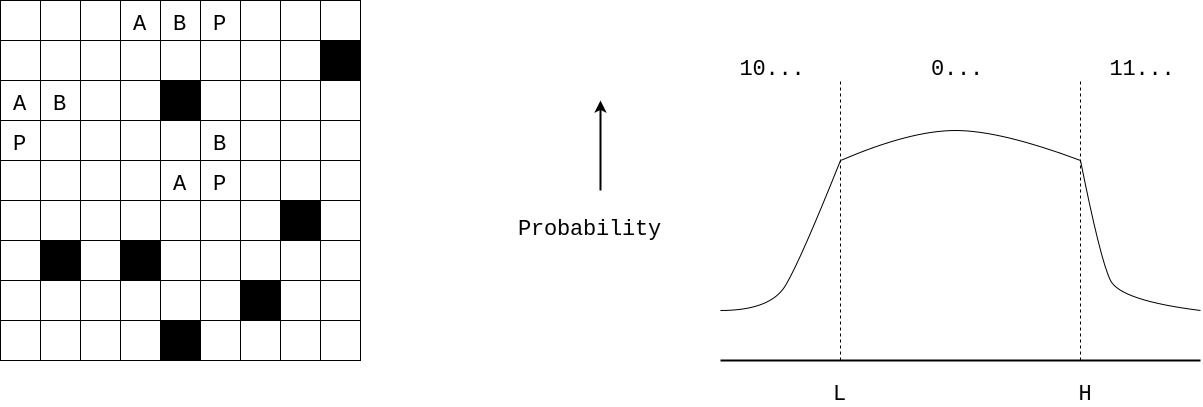
\includegraphics[width=7cm]{./Images/5.2.png}
\end{figure}
\FloatBarrier

\subsubsection{Torniamo alla Prova del
Pumping Lemma}
Sappiamo che il parse tree per z ha un
cammino con almeno $\mathrm{m}+1$ variabili.

Consideriamo il cammino più lungo.
Ci sono solo m variabili distinte, quindi
tra le m+1 più in basso possiamo trovare
due nodi con la stessa etichetta, diciamo
A. 

Il parse tree ha allora la forma:

\begin{figure}[hbpt!]
    \centering
    \includegraphics[width=10cm]{./Images/5.3.png}
\end{figure}
\FloatBarrier

\subsubsection{"Pump" zero volte}

\begin{figure}[hbpt!]
    \centering
    \includegraphics[width=8cm]{./Images/5.4.png}
\end{figure}
\FloatBarrier

\subsubsection{Iteriamo due volte}

\begin{figure}[hbpt!]
    \centering
    \includegraphics[width=8cm]{./Images/5.5.png}
\end{figure}
\FloatBarrier

\subsubsection{Iteriamo 3+ volte}

\begin{figure}[hbpt!]
    \centering
    \includegraphics[width=8cm]{./Images/5.6.png}
\end{figure}
\FloatBarrier

\subsubsection{Uso del Pumping Lemma}

$\left\{0^{i} 10^{i} \mid i \geq 1\right\}$ è un CFL.
Ma $\mathrm{~L}=\left\{0^{i} 10^{i} 10^{i} \mid i \geq 1\right\}$ non lo è. Lo proviamo usando il pumping lemma.

Supponiamo che L sia un CFL.

Sia n la costante del pumping lemma per L.

Consideriamo $z=0^{n} 10^{n} 10^{n} .$
Scriviamo z = uvwxy, dove
$|v w x| \leq n$ e $|v x| \geq 1 .$
\begin{itemize}
    \item \textbf{Caso 1:} vx non ha occorrenze di $0 .$
Almeno uno tra v e x è 1 e uwy ha al più un 1 , ma nessuna stringa in $L$ ha questa proprietà.
    \item \textbf{Caso 2:} vx ha almeno uno $0 .$ vwx è troppo corta (lunghezza $\leq \mathrm{n}$ ) per
essere fattore di tutti e tre i blocchi di 0 in
$0^{n} 10^{n} 10^{n} .$ Allora uwy ha almeno un blocco di n zeri e
almeno un blocco con meno di n zeri. Quindi, uwy non appartiene a L.
\end{itemize}

\subsubsection{Definizione di Forma Normale di Chomsky}

Una grammatica context-free $G=(V, \Sigma, P, S)$ è in forma normale di Chomsky (o in CNF) se ogni sua produzione ha la forma
\begin{enumerate}
    \item $A \rightarrow B C \operatorname{con} A, B, C \in V$,
    \item $A \rightarrow a \operatorname{con} A \in V e a \in \Sigma$,
    \item $S \rightarrow \epsilon$
\end{enumerate}

Inoltre, se $S \rightarrow \epsilon$ è in $P$, allora $B, C \in V \backslash\{S\}$ in (i).

\vspace{5mm}

\textbf{Teorema}

Per ogni grammatica context-free $G$ esiste una grammatica $G^{\prime}$ tale che $L\left(G^{\prime}\right)=L(G)$ e $G^{\prime}$ è in forma normale di Chomsky.

\vspace{5mm}

Se $G=(V, \Sigma, P, S)$ è una grammatica context-free in forma normale di Chomsky e w è una stringa in $L(G)$ di lunghezza $n \geq 1$, allora ogni derivazione di $w$ richiede esattamente $2 n-1$ passi.

\vspace{5mm}

Sia $G=(V, \Sigma, P, S)$ una grammatica context-free in forma normale di Chomsky. Se $w$ è una stringa in $\Sigma^{*}$ di lunghezza $n \geq 1$ derivabile da $A \in V$, il numero dei passi in $A \stackrel{*}{\Rightarrow} w$ è $2 n-1$.

\vspace{5mm}

\textbf{Prova. }

Sia $G=(V, \Sigma, P, S)$ una CFG in CNF e sia $A \Rightarrow w$, con $w \in \Sigma^{*}, A \in V$ e $|w|=n, n \geq 1$. La prova è per induzione su $n$.

\vspace{5mm}

\textbf{Passo Base.} Sia $n=1$, quindi $w=a \in \Sigma$ e $2 n-1=1$. Per definizione di CNF, $A \rightarrow a \in P$ e la derivazione $A \Rightarrow w$ è una derivazione in un passo $A \Rightarrow a$ (derivazione diretta).

\vspace{5mm}

\textbf{Passo Induttivo.} Sia $n>1$, sia $A \stackrel{*}{\Rightarrow} w$ una derivazione di $w$ da $A$. Per definizione di CNF, esistono $B, C \in V$ tali che
$$
A \Rightarrow B C \stackrel{*}{\Rightarrow} w
$$

Per una proprietà delle CFG, esistono $w_{1}, w_{2}$ tali che $w=w_{1} w_{2}$ e
$$
B \stackrel{*}{\Rightarrow} w_{1}, \quad C \stackrel{*}{\Rightarrow} w_{2}, \quad A \Rightarrow B C \stackrel{*}{\Rightarrow} w_{1} C \stackrel{*}{\rightarrow} w
$$

Inoltre, $1<\left|w_{1}\right|<|w|, 1<\left|w_{2}\right|<|w|$ e $t=1+t_{1}+t_{2}$, dove $t$ è il numero dei passi in $A \Rightarrow w, t_{1}$ è il numero dei passi in $B \stackrel{*}{\Rightarrow} w_{1}$ e $t_{2}$ è il numero dei passi in $C \stackrel{*}{\Rightarrow} w_{2}$.

Applicando l'ipotesi induttiva abbiamo
$$
\begin{aligned}
t &=1+t_{1}+t_{2} \\
&=1+2\left|w_{1}\right|-1+2\left|w_{2}\right|-1 \\
&=2\left(\left|w_{1}\right|+\left|w_{2}\right|\right)-1=2|w|-1=2 n-1
\end{aligned}
$$
il che conclude la prova.

\subsubsection{Alberi sintattici}

Sia $G=(V, T, P, S)$ una grammatica context-free. Gli alberi sintattici (o parse tree) di G sono alberi che soddisfano le seguenti definizioni.
\begin{enumerate}
    \item Ciascun nodo interno è etichettato da una variabile in $V$.
    \item Ogni foglia è etichettata da una variabile o da un terminale o da $\epsilon$. Se una foglia ha come etichetta $\epsilon$, deve essere I'unico figlio del suo genitore.
    \item Se un nodo interno è etichettato $A$ e i suoi figli sono etichettati, a partire da sinistra,
$$
X_{1}, X_{2}, \ldots, X_{k}
$$
allora $A \rightarrow X_{1} X_{2}, \cdots X_{k}$ è una produzione in $P$. Se esiste $i$, $1 \leq i \leq k$, tale che $X_{i}=\epsilon$, allora $k=1$ e $A \rightarrow \epsilon \in P$ (per la precedente condizione).
\end{enumerate}

Gli alberi sintattici di una grammatica context-free $G$ in forma normale di Chomsky sono alberi binari (ogni nodo ha al più due figli).

Inoltre, se $w \in L(G), w \neq \epsilon$, l'albero sintattico di $G$ con prodotto $w$ ha nodi interni etichettati da variabili e le foglie etichettate dalle lettere che compongono $w$. Tutti i nodi interni hanno due figli, tranne i genitori delle foglie. I genitori delle foglie hanno un solo figlio.

\subsubsection{Dimensione degli alberi sintattici}

\textbf{Teorema}

Sia $G=(V, \Sigma, P, S)$ una grammatica context-free in forma normale di Chomsky. Sia $\mathcal{T}$ un albero sintattico in $G$ di radice $A \in V$ e prodotto $w \in \Sigma^{+} .$ Se la lunghezza del più lungo cammino in $\mathcal{T}$ è n, abbiamo $|w| \leq 2^{n-1}$.

La prova è per induzione su $n$.

\vspace{5mm}

\textbf{Passo Base:} $n=1$. Sia $\mathcal{T}$ un albero sintattico in $G$ di radice A e prodotto $w \in \Sigma^{+}$.
Ricordiamo che in un albero la lunghezza di un cammino è uguale al numero dei nodi che attraversa meno $1 .$
Se la lunghezza del più lungo cammino in $\mathcal{T}$ è $n=1, \mathcal{T}$ è costituito dalla radice $A$ che ha un sol figlio, una foglia.
Quindi $A \Rightarrow w$ e $|w|=1=2^{0}=2^{n-1}$.

\vspace{5mm}

\textbf{Passo Induttivo:} Sia $\mathcal{T}$ un albero sintattico in $G$ di radice $A$ e prodotto $w \in \Sigma^{+}$. Supponiamo che la lunghezza del più lungo cammino in $\mathcal{T}$ sia $n>1$.
La radice di $\mathcal{T}$ ha due figli $B, C \in V$ e $A \rightarrow B C \in P .$
Inoltre, il sottoalbero $\mathcal{T}_{1} \mathrm{di} \mathcal{T}$ radicato in $B$ è un albero sintattico. Sia $n_{1}$ la lunghezza del più lungo cammino in $\mathcal{T}_{1}$ e sia $w_{1}$ il suo prodotto.
II sottoalbero $\mathcal{T}_{2}$ di $\mathcal{T}$ radicato in $C$ è un albero sintattico. Sia $n_{2}$ la lunghezza del più lungo cammino in $\mathcal{T}_{2}$ e sia $w_{2}$ il suo prodotto.
Risulta $w=w_{1} w_{2}, n_{1} \leq n-1, n_{2} \leq n-1$ e quindi, per ipotesi induttiva, $\left|w_{1}\right| \leq 2^{n_{1}-1},\left|w_{2}\right| \leq 2^{n_{2}-1}$.
In conclusione:
$$
|w|=\left|w_{1}\right|+\left|w_{2}\right| \leq 2^{n_{1}-1}+2^{n_{2}-1} \leq 2^{n-2}+2^{n-2}=2^{n-1}
$$

\subsubsection{Pumping lemma per i CFL}

\textbf{Teorema}

Sia $L$ è un linguaggio context-free. Esiste un numero $n$ (lunghezza del pumping) tale che se z è una stringa di L di lunghezza almeno $n$, possiamo scrivere $z=u v w x y$ con le seguenti condizioni:
\begin{enumerate}
    \item per ogni $i \geq 0$, $u v^{i} w x^{i} y \in L$
    \item $|v x|>0$
    \item  $|v w x| \leq n$
\end{enumerate}

Sia $G=(V, \Sigma, P, S)$ una grammatica context-free in forma normale di Chomsky tale che $L=L(G)$.

Faremo vedere che esiste $n$ per cui ogni stringa $z \in L(G)$, con $|z| \geq n$ ha una derivazione della forma
$$
S \stackrel{*}{\Rightarrow} u \mathrm{~A} y \stackrel{*}{\Rightarrow} u v A x y \stackrel{*}{\Rightarrow} u v w x y
$$
per qualche $A \in V$ e $v x \neq \epsilon$.
La condizione (1) segue immediatamente ripetendo un numero qualsiasi $i 
\geq 0$ di volte la (sotto-) derivazione $A \stackrel{*}{\Rightarrow} v A x$.

\vspace{5mm}

Sia $m=|V|$ e sia $n=2^{m} .$ Sia $z \in L(G)$ con $|z| \geq n=2^{m} .$ Ogni albero sintattico $\mathcal{T}$ con radice $S$ e prodotto $z$ ha un cammino $c$, con $|c| \geq m+1$ (altrimenti il più lungo cammino $c$ ha lunghezza $|c| \leq m$ e $\left.|z| \leq 2^{m-1}<n\right)$.

In $\mathcal{T}$ c'è un cammino piú lungo di $m$ e quindi c'è una variabile, sia $A$, che appare due volte. Scegliamo $A$ in modo che sia una variabile che si ripete tra le $|V|+1$ variabili più in basso su questo cammino.

Il sotto-albero di $\mathcal{T}$ radicato in $A$ corrisponde alla derivazione $A \stackrel{*}{\Rightarrow} v A x$.

Risulta $|v w x| \leq n=2^{m}$ (prodotto di albero sintattico con cammino più lungo $m+1$ ) e $v x \neq \epsilon$ (per definizione di grammatica context-free in CNF).

\vspace{5mm}

II linguaggio
$$
B=\left\{a^{n} b^{n} c^{n} \mid n \geq 0\right\}
$$
non è context-free.

\vspace{5mm}

Supponiamo per assurdo che $B=\left\{a^{n} b^{n} C^{n} \mid n \geq 0\right\}$ sia context-free.

Allora $B$ verifica il pumping lemma, sia $n$ la costante del pumping.

Siccome $a^{n} b^{n} c^{n} \in B$ e $\left|a^{n} b^{n} c^{n}\right| \geq n$, esiste una divisione $a^{n} b^{n} c^{n}=u v w x y$ che verifica le condizioni $(1),(2)$ e (3) del lemma.
La stringa vwx non può contenere sia a che c poiché l'ultima a e la prima $c$ sono separate da $n$ caratteri uguali a $b$ e $|v w x| \leq n .$ Ci sono due casi
\begin{enumerate}
    \item $v w x$ non contiene $c:\left|u v^{2} w x^{2} y\right|_{c}=n \operatorname{ma}\left|u v^{2} w x^{2} y\right|_{a}$ oppure $\left|u v^{2} w x^{2} y\right|_{b}$ è maggiore di $n$.
    \item $v w x$ non contiene $a:\left|u v^{2} w x^{2} y\right|_{a}=n$ ma $\left|u v^{2} w x^{2} y\right|_{b}$ oppure $\left|u v^{2} w x^{2} y\right|_{c}$ è maggiore di $n$.
\end{enumerate}

Quindi $u v^{2} w x^{2} y \notin L(G)$, assurdo.

\subsubsection{Gerarchia di Chomsky}

Il linguaggio
$$
B=\left\{a^{n} b^{n} c^{n} \mid n \geq 0\right\}
$$
non è context-free ma è di tipo $1 .$
Infatti $B=L(G)$ dove $G=(V, T, P, S), V=\{S, B\}$, $T=\{a, b, c\}$ e $P$ consiste nelle seguenti produzioni
\begin{enumerate}
    \item $S \rightarrow a S B c \mid a b c$
    \item $c B \rightarrow B C$
    \item $b B \rightarrow b b$
\end{enumerate}

\subsubsection{Proprietà dei linguaggi context-free}
\begin{itemize}
    \item $\left\{a^{m} b^{n} c^{n} \mid n, m \geq 0\right\}$ è context-free, è generato da una CFG con produzioni
$$
S \rightarrow S_{1} S_{2}, \quad S_{1} \rightarrow a S_{1}\left|\epsilon, \quad S_{2} \rightarrow b S_{2} c\right| \epsilon
$$
    \item $\left\{a^{n} b^{n} c^{m} \mid n, m \geq 0\right\}$ è context-free, è generato da una CFG con produzioni
$$
X \rightarrow X_{1} X_{2}, \quad X_{1} \rightarrow a X_{1} b\left|\epsilon, \quad X_{2} \rightarrow c X_{2}\right| \epsilon
$$
    \item Il linguaggio
$$
\left\{a^{n} b^{n} c^{n} \mid n \geq 0\right\}=\left\{a^{m} b^{n} c^{n} \mid n, m \geq 0\right\} \cap\left\{a^{n} b^{n} c^{m} \mid n, m \geq 0\right\}
$$
non è context-free.
\end{itemize}

\subsubsection{Proprietà di chiusura}

La classe dei linguaggi context-free è chiusa rispetto all'unione, alla concatenazione e all'operazione star di Kleene.
Se $X$ ed $Y$ sono linguaggi context-free allora
\begin{itemize}
    \item $X \cup Y$ è un linguaggio context-free,
    \item $X Y$ è un linguaggio context-free,
    \item $X^{*}$ è un linguaggio context-free.
\end{itemize}

La classe dei linguaggi context-free non è chiusa rispetto all'intersezione.
Abbiamo visto un esempio di linguaggio non context-free che è intersezione di due linguaggi context-free.

Dati due insiemi $X$ e Y, risulta
$$
X \cap Y=\overline{\bar{X} \cap \bar{Y}}=\overline{\bar{X} \cup \bar{Y}}
$$

La classe dei linguaggi context-free non è chiusa rispetto al complemento.
Se $X$ è un linguaggio context-free, $\bar{X}$ può non essere context-free.

\vspace{5mm}

Se $X$ è un linguaggio context-free e $Y$ è un linguaggio regolare, allora $X \cap Y$ è un linguaggio context-free.

I linguaggi context-free deterministici sono chiusi rispetto al complemento.

\subsubsection{Linguaggi formali e di programmazione}

$$
\begin{aligned}
&L_{1}=\left\{w C w \mid w \in\{a, b\}^{+}\right\} \\
&L_{1}^{\prime}=\left\{a^{n} b^{m} c^{n} d^{m} \mid n, m \geq 1\right\}
\end{aligned}
$$

Un'interpretazione di $L_{1}$ vede il prefisso $w$ come la dichiarazione di un identificatore con tale nome, c come (una parte di) un programma, e il suffisso $w$ come l'uso dell'identificatore medesimo.

Per quanto riguarda le stringhe di $L_{1}^{\prime}$ potremmo supporre di avere due procedure con $n$ ed $m$ parametri rispettivamente. Allora possiamo interpretare $a^{n}$ e $b^{m}$ come i parametri formali che appaiono nella dichiarazione delle procedure in questione e $c^{n} e d^{m}$ come i parametri attuali delle loro chiamate.

\vspace{5mm}

$$
\begin{aligned}
L &=\left\{w w \mid w \in\{a, b\}^{+}\right\} \\
L_{1} &=\left\{w c w \mid w \in\{a, b\}^{+}\right\} \\
L_{1}^{\prime} &=\left\{a^{n} b^{m} c^{n} d^{m} \mid n, m \geq 1\right\}
\end{aligned}
$$
Questi linguaggi non sono context-free.

\begin{itemize}
    \item $L_{1}^{\prime}=\left\{a^{n} b^{m} c^{n} d^{m} \mid n, m \geq 1\right\}$ non è context-free: applicare il pumping lemma alla stringa $a^{n} b^{n} c^{n} d^{n}$ con $n$ uguale alla lunghezza del pumping.
    \item $L=\left\{w w \mid w \in\{a, b\}^{+}\right\}$non è context-free: se lo fosse lo sarebbe anche $L \cap a^{+} b^{+} a^{+} b^{+}=\left\{a^{n} b^{m} a^{n} b^{m} \mid n, m \geq 1\right\}=X$. Ma $X$ non verifica il pumping lemma per i linguaggi context-free.
    \item  $L_{1}=\left\{w c w \mid w \in\{a, b\}^{+}\right\}$non è context-free: se lo fosse lo sarebbe anche
$$
L_{1} \cap a^{+} b^{+} c a^{+} b^{+}=\left\{a^{n} b^{m} c a^{n} b^{m} \mid n, m \geq 1\right\}=Y
$$
Ma Y non verifica il pumping lemma per i linguaggi context-free.
\end{itemize}

\subsubsection{Pumping lemma per i linguaggi context-free}

Il pumping lemma stabilisce una condizione necessaria affinché un
linguaggio sia context-free.
Se un linguaggio verifica il pumping lemma non è detto che sia
context-free.

\vspace{5mm}

Il linguaggio
$$
\begin{aligned}
L &=\left\{a^{i} b^{j} c^{k} d^{\ell} \mid i, j, k, \ell \in \mathbb{N}, i=0 \text { oppure } j=k=\ell\right\} \\
&=L\left(b^{*} c^{*} d^{*}\right) \cup\left\{a^{i} b^{j} c^{j} d^{j} \mid i, j \in \mathbb{N}, i>0, j \geq 0\right\}
\end{aligned}
$$
verifica il pumping lemma ma non è context-free.
$L$ verifica una versione più forte del pumping lemma, detta
\textbf{Lemma di Odgen}





\let\cleardoublepage\clearpage

